\documentclass[14pt, a4paper]{extarticle}
\usepackage{fefu_title}

\titlelabel{\thetitle.\quad}

\graphicspath{{./}}
\DeclareGraphicsExtensions{.png, .jpg}

\renewcommand{\cftsecleader}{\cftdotfill{\cftdotsep}}
\let \savenumberline \numberline
\def \numberline#1{\savenumberline{#1.}}

\counterwithin*{equation}{section}

\lstset{
	basicstyle=\fontsize{9}{9}\selectfont\ttfamily
}

\begin{document}
	
	\fefutitlepage{Б8118-02.03.01сцт}{Мышалов Р.Е.}{30}{мая}{2020}
	
	\tableofcontents
	\pagebreak
	
	\section{Введение}
		В данной лабораторной работе нам предстоит дать характеристику предоставленным уравнениям, используя полученные знания, а также написать программный код для численного нахождения значения функции в точке с помощью метода Эйлера. 
	\pagebreak
	
	\section{Дать характеристику уравнениям, найти общее решение и нарисовать векторное поле}
		\begin{enumerate}
			\item \(\dfrac{y}{y'^{2}} = 1 - \tg y'\) 
			
				Характеристика: уравнение не содержит \(x\)
				
				Общее решение:
				\begin{align*}
					\begin{cases}
						x = 2p - p\tg p - \ln \left|\cos p\right| + C \\
						y = p^2 (1 - \tg p)
					\end{cases}
				\end{align*}
				
				Векторного поля нет.
				
			\item \(y'^{3} - 2xy'^{2} + y' = 2x\)
				
				Характеристика: уравнение не содержит $y$ в явном виде, а также является кубическим относительно $y'$
				
				Общее решение: \(y(x) = C + x^{2}\)
				
				Векторного поля нет.
				
			\item \(y'^{2} - \dfrac{1 + \sin 2x}{e^{2y}} = 0\)
			
				Характеристика: уравнение, разрешённое относительно производной
			
				Общее решение: \( y(x) = \ln\left(C + \dfrac{\sqrt{2\sin x \cos x - 1} \pm \left( \cos x - \sin x\right)}{\sin x + \cos x}\right)\)
			
				Векторное поле:

				\hspace{-1cm}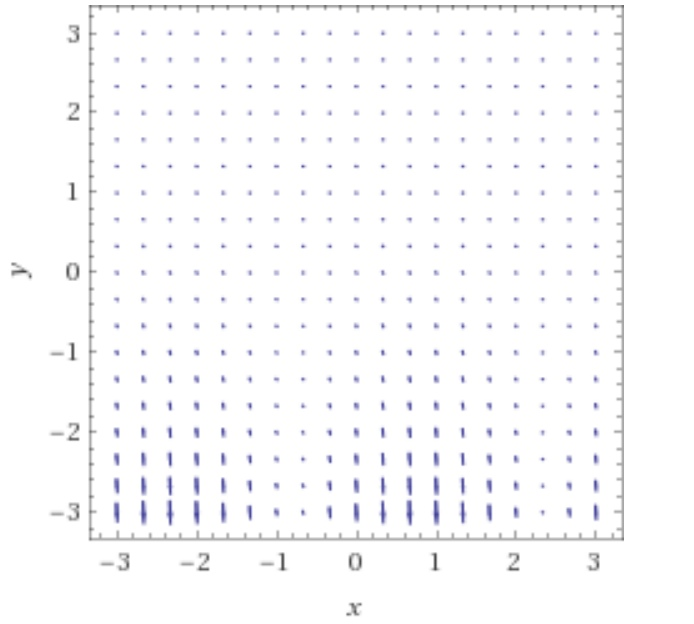
\includegraphics[width=8.5cm]{vector_3}
				\pagebreak
				
			\item \(y = \dfrac{3}{2} xy' + e^{y'}\)
			
				Характеристика: уравнение Лагранжа
			
				Общее решение:
					\begin{align*}
						\begin{cases}
							 x = e^p \cdot \left(-4p^{-3}+4p^{-2}-2p^{-1}\right) + Cp^{-3}\\
							 y = \dfrac{3}{2} \left(e^p \cdot \left(-4p^{-2}+4p^{-1}-2\right)+p^{-2}C\right) + e^p
						\end{cases}
					\end{align*}
			
				Векторного поля нет.
				
			\item \(\dfrac{y}{y'} = x + \sqrt{1 + \dfrac{1}{y'^2}}\)

				Характеристика: уравнение Клеро
			
				Общее решение: \(y(x) = C \left(x + \sqrt{\dfrac{1}{C^2} + 1}\right)\)
			
				Векторного поля нет.
		\end{enumerate}
		\pagebreak
		
		\section{Разрешить уравнения относительно производной, найти значение функции в точке и нарисовать график}
			\begin{enumerate}
				\item \(xy' - y^2 \cdot e^{-y^2} = \sin {\pi x}; \qquad y(1) = \ln 2, \quad y(\pi) = \mathcal{?}\)
					
					\(y' = \dfrac{\sin {\pi x} + y^2 \cdot e^{-y^2}}{x}; \qquad y(\pi) = 0.7858612098160048\)
					
					\hspace{-1cm}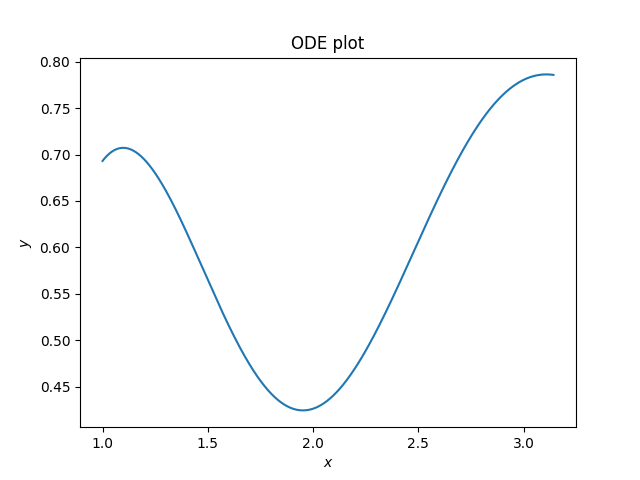
\includegraphics[width=11cm]{plot_1}
					
				\item \(\sin(\ln x - xy) + \tg(y' - 1) = x; \quad y(\ln 2) = -\pi, y\left({e^{-2}}\right) = ?\)
					
					\(y' = \arcsin {\left(x - \sin {\left(\ln x - y\right)}\right)} + 1; \quad y(\ln 2) = -3.7517706910266035\)
					
					\hspace{-1cm}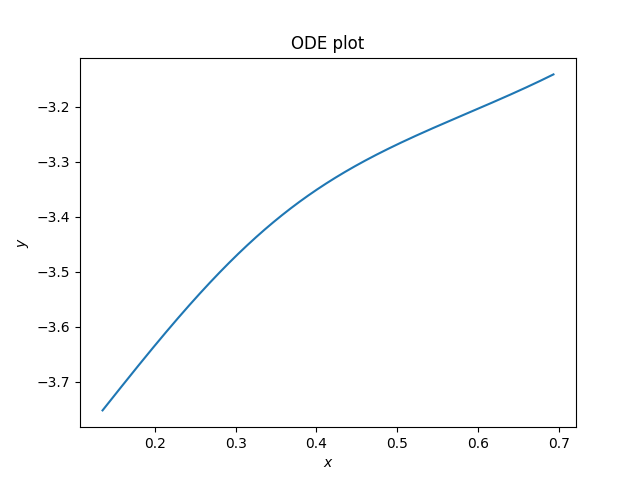
\includegraphics[width=11cm]{plot_2}
					
					\pagebreak
					\begin{lstlisting}[language=Python, frame=single, gobble=12, tabsize=2]
						import matplotlib.pyplot as plt
						from math import sin, pi, exp, log, atan
						
						class ODE:
							_plot_is_created = False
							_values_are_calculated = False
						
							def __init__(self, initial_x, initial_y):
								self._x = initial_x
								self._y = initial_y
								_x_values = []
								_y_values = []
						
							def __diff_value(self):
								if (self._task_number == 1):
									return (sin(pi * self._x) + self._y**2 * exp(-self._y**2))/self._x
								if (self._task_number == 2):
									return (atan(self._x - sin(log(self._x) - self._x * self._y)) + 1)
						
							def find_y_euler(self, step, searched_point_x):
								if (self._task_number == 1):
									while(self._x < searched_point_x):
										self._y = self._y + self.__diff_value() * step
										self._x += step
										self._x_values.append(self._x)
										self._y_values.append(self._y)
								if (self._task_number == 2):
									while(self._x > searched_point_x):
										self._y = self._y - self.__diff_value() * step
										self._x -= step
										self._x_values.append(self._x)
										self._y_values.append(self._y)
								self._values_are_calculated = True
								return self._y
						
							def create_plot(self):
								if (self._values_are_calculated):
									plt.plot(self._x_values, self._y_values)
									plt.xlabel('$x$')
									plt.ylabel('$y$')
									plt.title("ODE plot")
									self._plot_is_created = True
								else:
									print("There are no values to plot!")
						
							def show_plot(self):
								if (not self._plot_is_created):
									self.create_plot()
								plt.show()
						
							def save_plot(self, name, extension):
								if (self._plot_is_created):
									plt.savefig(f'{name}.{extension}')
									plt.close()
								else:
									print("Plot doesn't exist!")
						
							def main():
								ode1 = ODE(1, log(2), 1)
								result1 = ode1.find_y_euler(0.00001, pi)
								ode1.create_plot()
								ode1.save_plot('plot_1', 'png')
								
								ode2 = ODE(log(2), -pi, 2)
								result2 = ode2.find_y_euler(0.00001, 1/exp(2))
								ode2.create_plot()
								ode2.save_plot('plot_2', 'png')
								print(result1, result2)
								
							if __name__ == "__main__":
								main()
					\end{lstlisting}
			\end{enumerate}
			\pagebreak
			
		\section{Для следующих дифференциальных уравнений определить тип, дать характеристику, и с помощью программ компьютерной математики найти общее решение}
			\begin{enumerate}
				\item \(y'' \cdot \cos y + y'^2 \cdot \sin y = y'\)
				
					Тип: уравнение,  допускающее понижение порядка
					
					Характеристика: уравнение не содержит независимого аргумента
					
					Общее решение: \[ \dfrac{\ln\left(\left|C_1\tan\left(\frac{y}{2}\right)+\sqrt{C_1^2+1}-1\right|\right)-\ln\left(\left|C_1\tan\left(\frac{y}{2}\right)-\sqrt{C_1^2+1}-1\right|\right)}{\sqrt{C_1^2+1}} = x + C_2\]
					
				\item \(yy'' + y'^2 = e^y(1+xy')\)
				
					Тип:  уравнение в полных производных
				
					Характеристика: уравнение разрешимое в производной
				
					Общее решение: \(e^{-y} = C_1^{-2} \cdot (C_1x - 1) + e^{-C_1x}C_2\)
					
				\item \(y'' \cdot \cos y = y'^2 \cdot \sin y + 1\)
				
					Тип: уравнение,  допускающее понижение порядка
					
					Характеристика: уравнение не содержит независимого аргумента
				
					Общее решение: \(y(x) = \pm \arcsin\left(0.25\left(2\sqrt{2} \cdot C_2x\pm \left(C_2^2 + 2x^2 - 2C_1\right)\right)\right)\)
			\end{enumerate}
\end{document}